\documentclass[12pt]{article}

\usepackage[utf8]{inputenc}
\usepackage{amsmath}
\usepackage{graphicx}
\usepackage{geometry}
\geometry{a4paper, margin=1in}
\usepackage{hyperref}
\newcommand{\note}[1]{\textbf{#1}} % Makes the term bold

\begin{document}

\begin{titlepage}
    \centering

    \vspace*{1cm}

    \rule{\textwidth}{1pt}

    \vspace{2\baselineskip}

    {\huge  Cyber Security } \\

    \vspace{1\baselineskip}

    {\huge \textbf{ Lab 2 - Exploring DNS Traffic }}

    \vspace{2\baselineskip}

    \rule{\textwidth}{1pt}

    \vspace{1cm}

    \large

    \begin{flushleft}
        \begin{minipage}{.8\textwidth}
            \raggedright
            Fullname: Amangeldi Zhanserik \\
            ID: 22B030301 \\
            E-mail: {\normalsize \url{zha_amangeldi@kbtu.kz}} \\
            Date of submission: \today \\
            Class time: Thursday, 15:00--18:00 \\
        \end{minipage}%
    \end{flushleft}

    \vspace{2cm}

    
\includegraphics[width=.7\textwidth]{logo-kbtu.png}

    \vfill

    School of Information System and Engineering \\
    Kazakh-British Technical University \\
    Academic Year 2024-2025 \\
\end{titlepage}


\section{Capture DNS Traffic}

\subsection{Download and install Wireshark.}

\begin{enumerate}
    \item I go to the \href{https://www.wireshark.org}{Wireshark website} and install version based my own system(MacOS). \\
    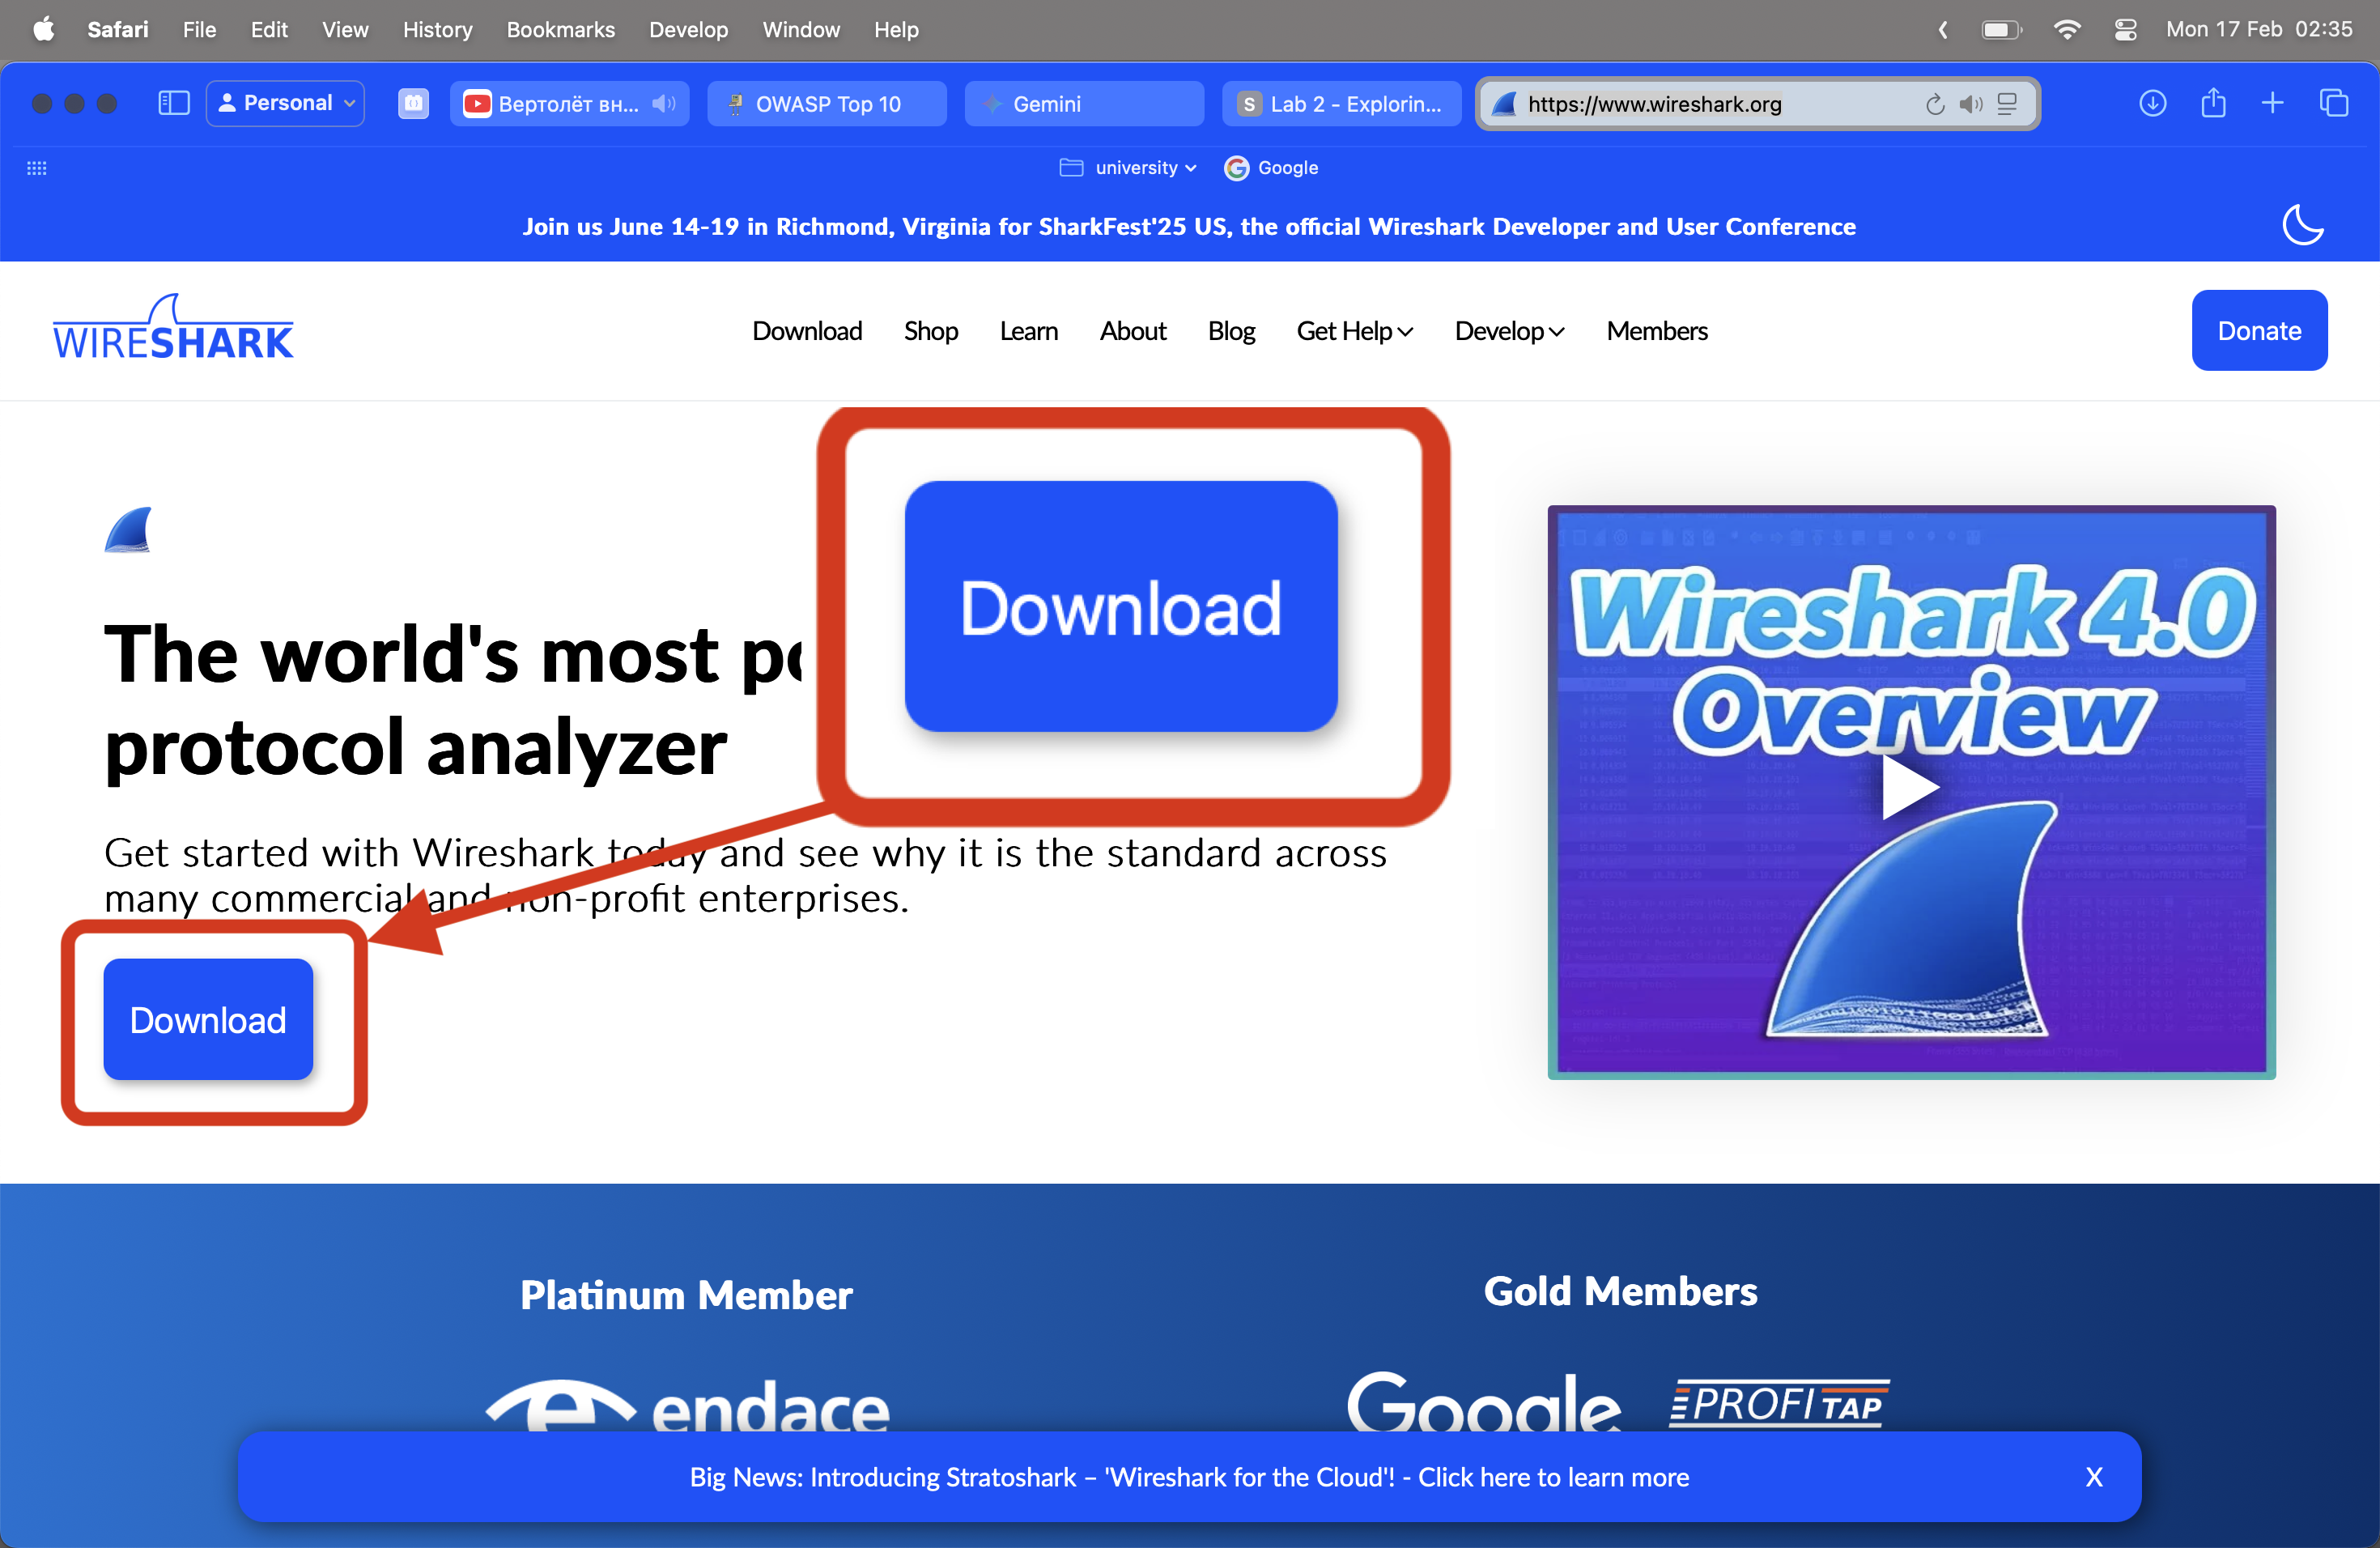
\includegraphics[width=.7\textwidth]{Image1.png} \\
    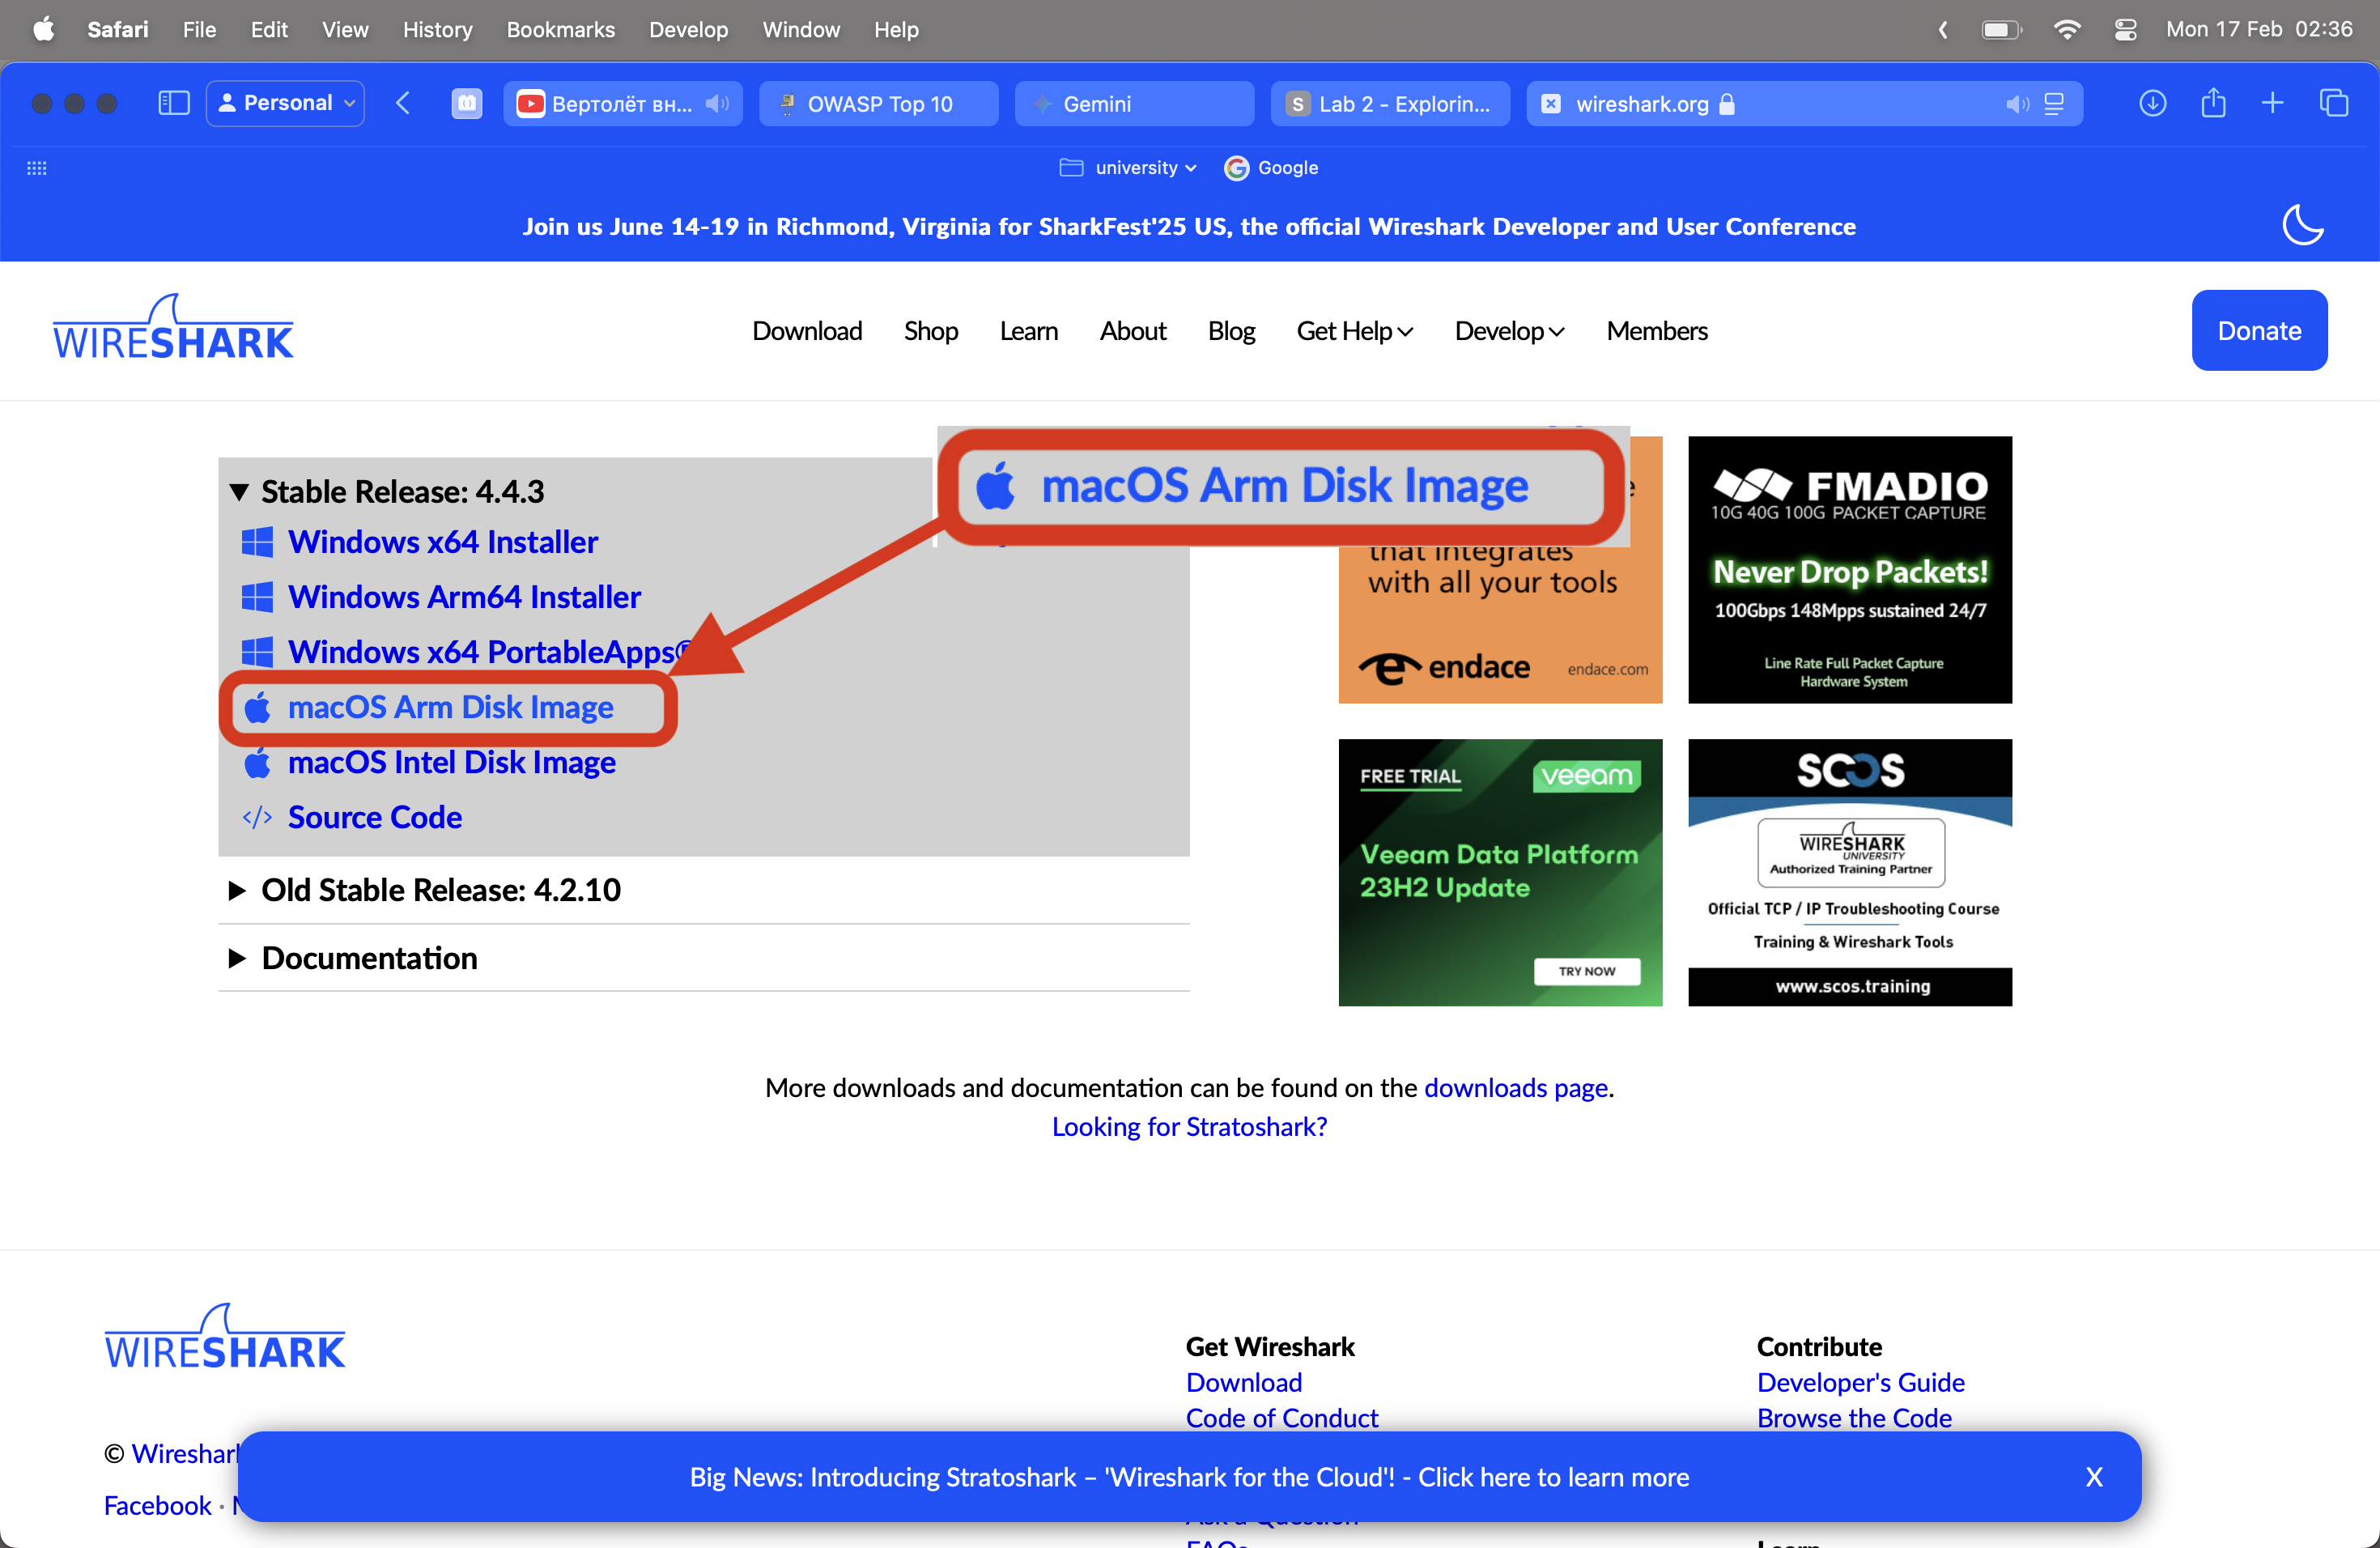
\includegraphics[width=.7\textwidth]{Image2.png} \\
    \item After downloading it, I open the downloaded file and install it. \\ 
    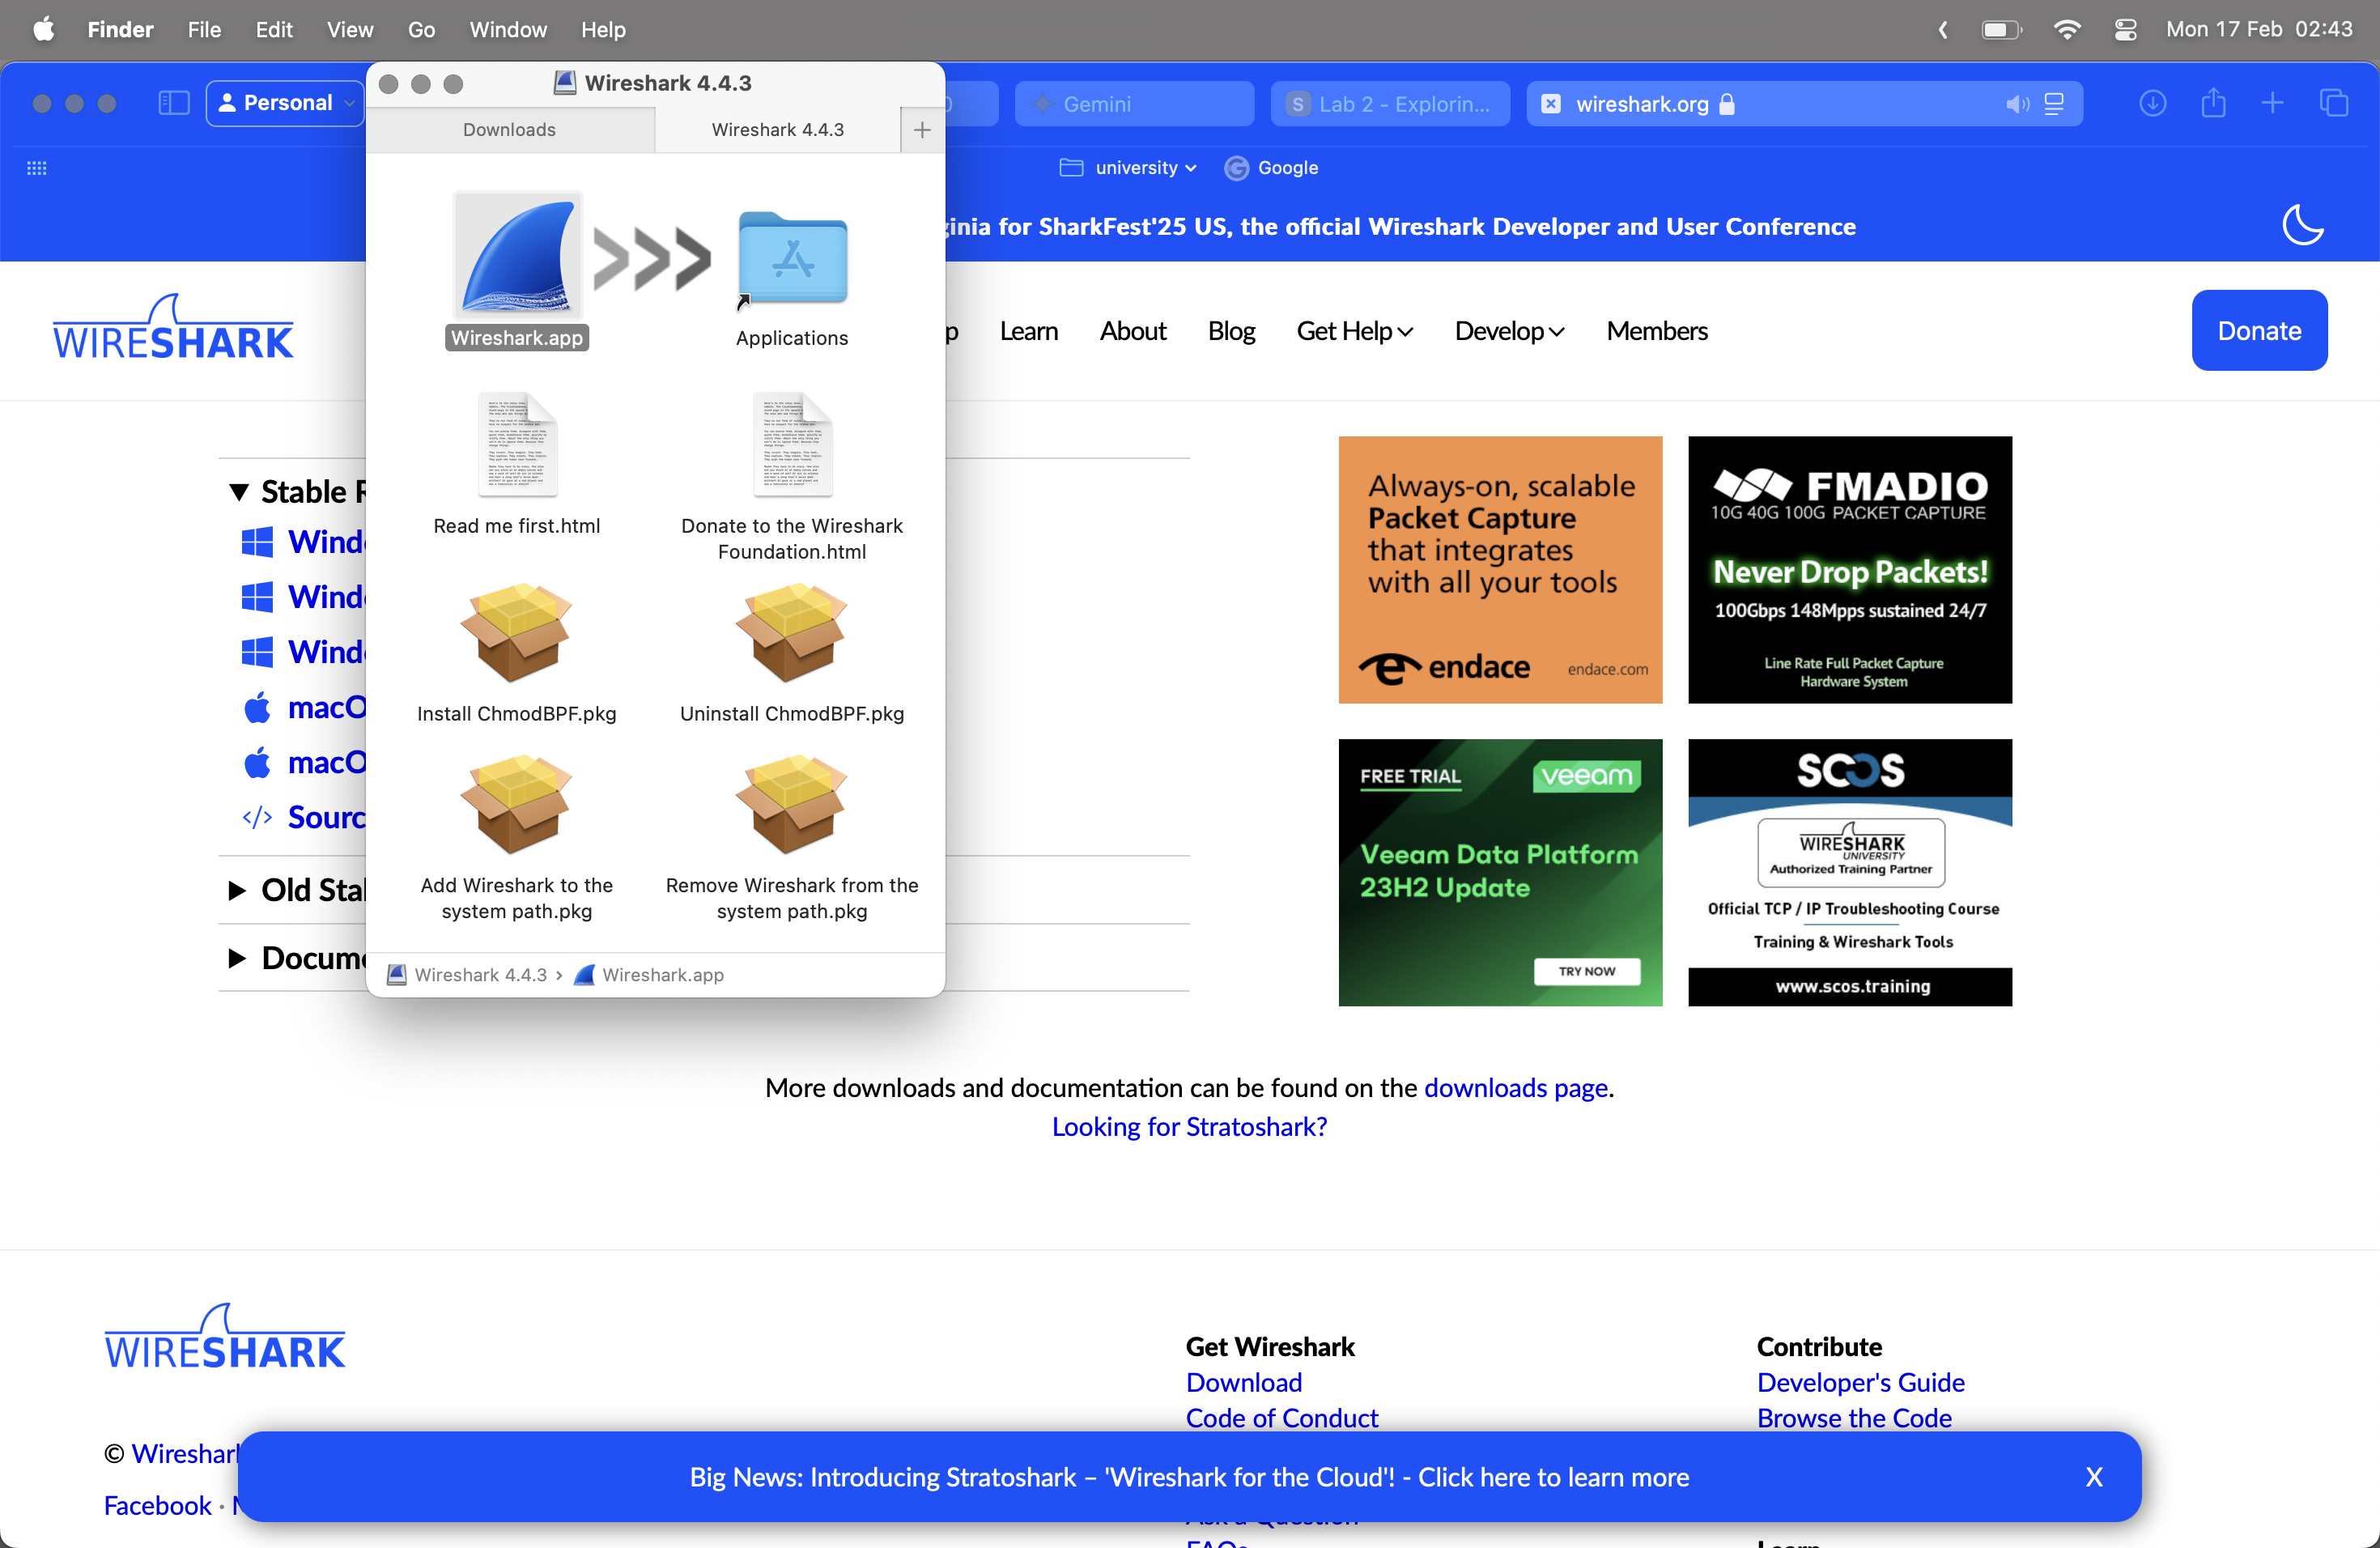
\includegraphics[width=.7\textwidth]{Image3.png} \\
    \item And open the Wireshark application. \\
    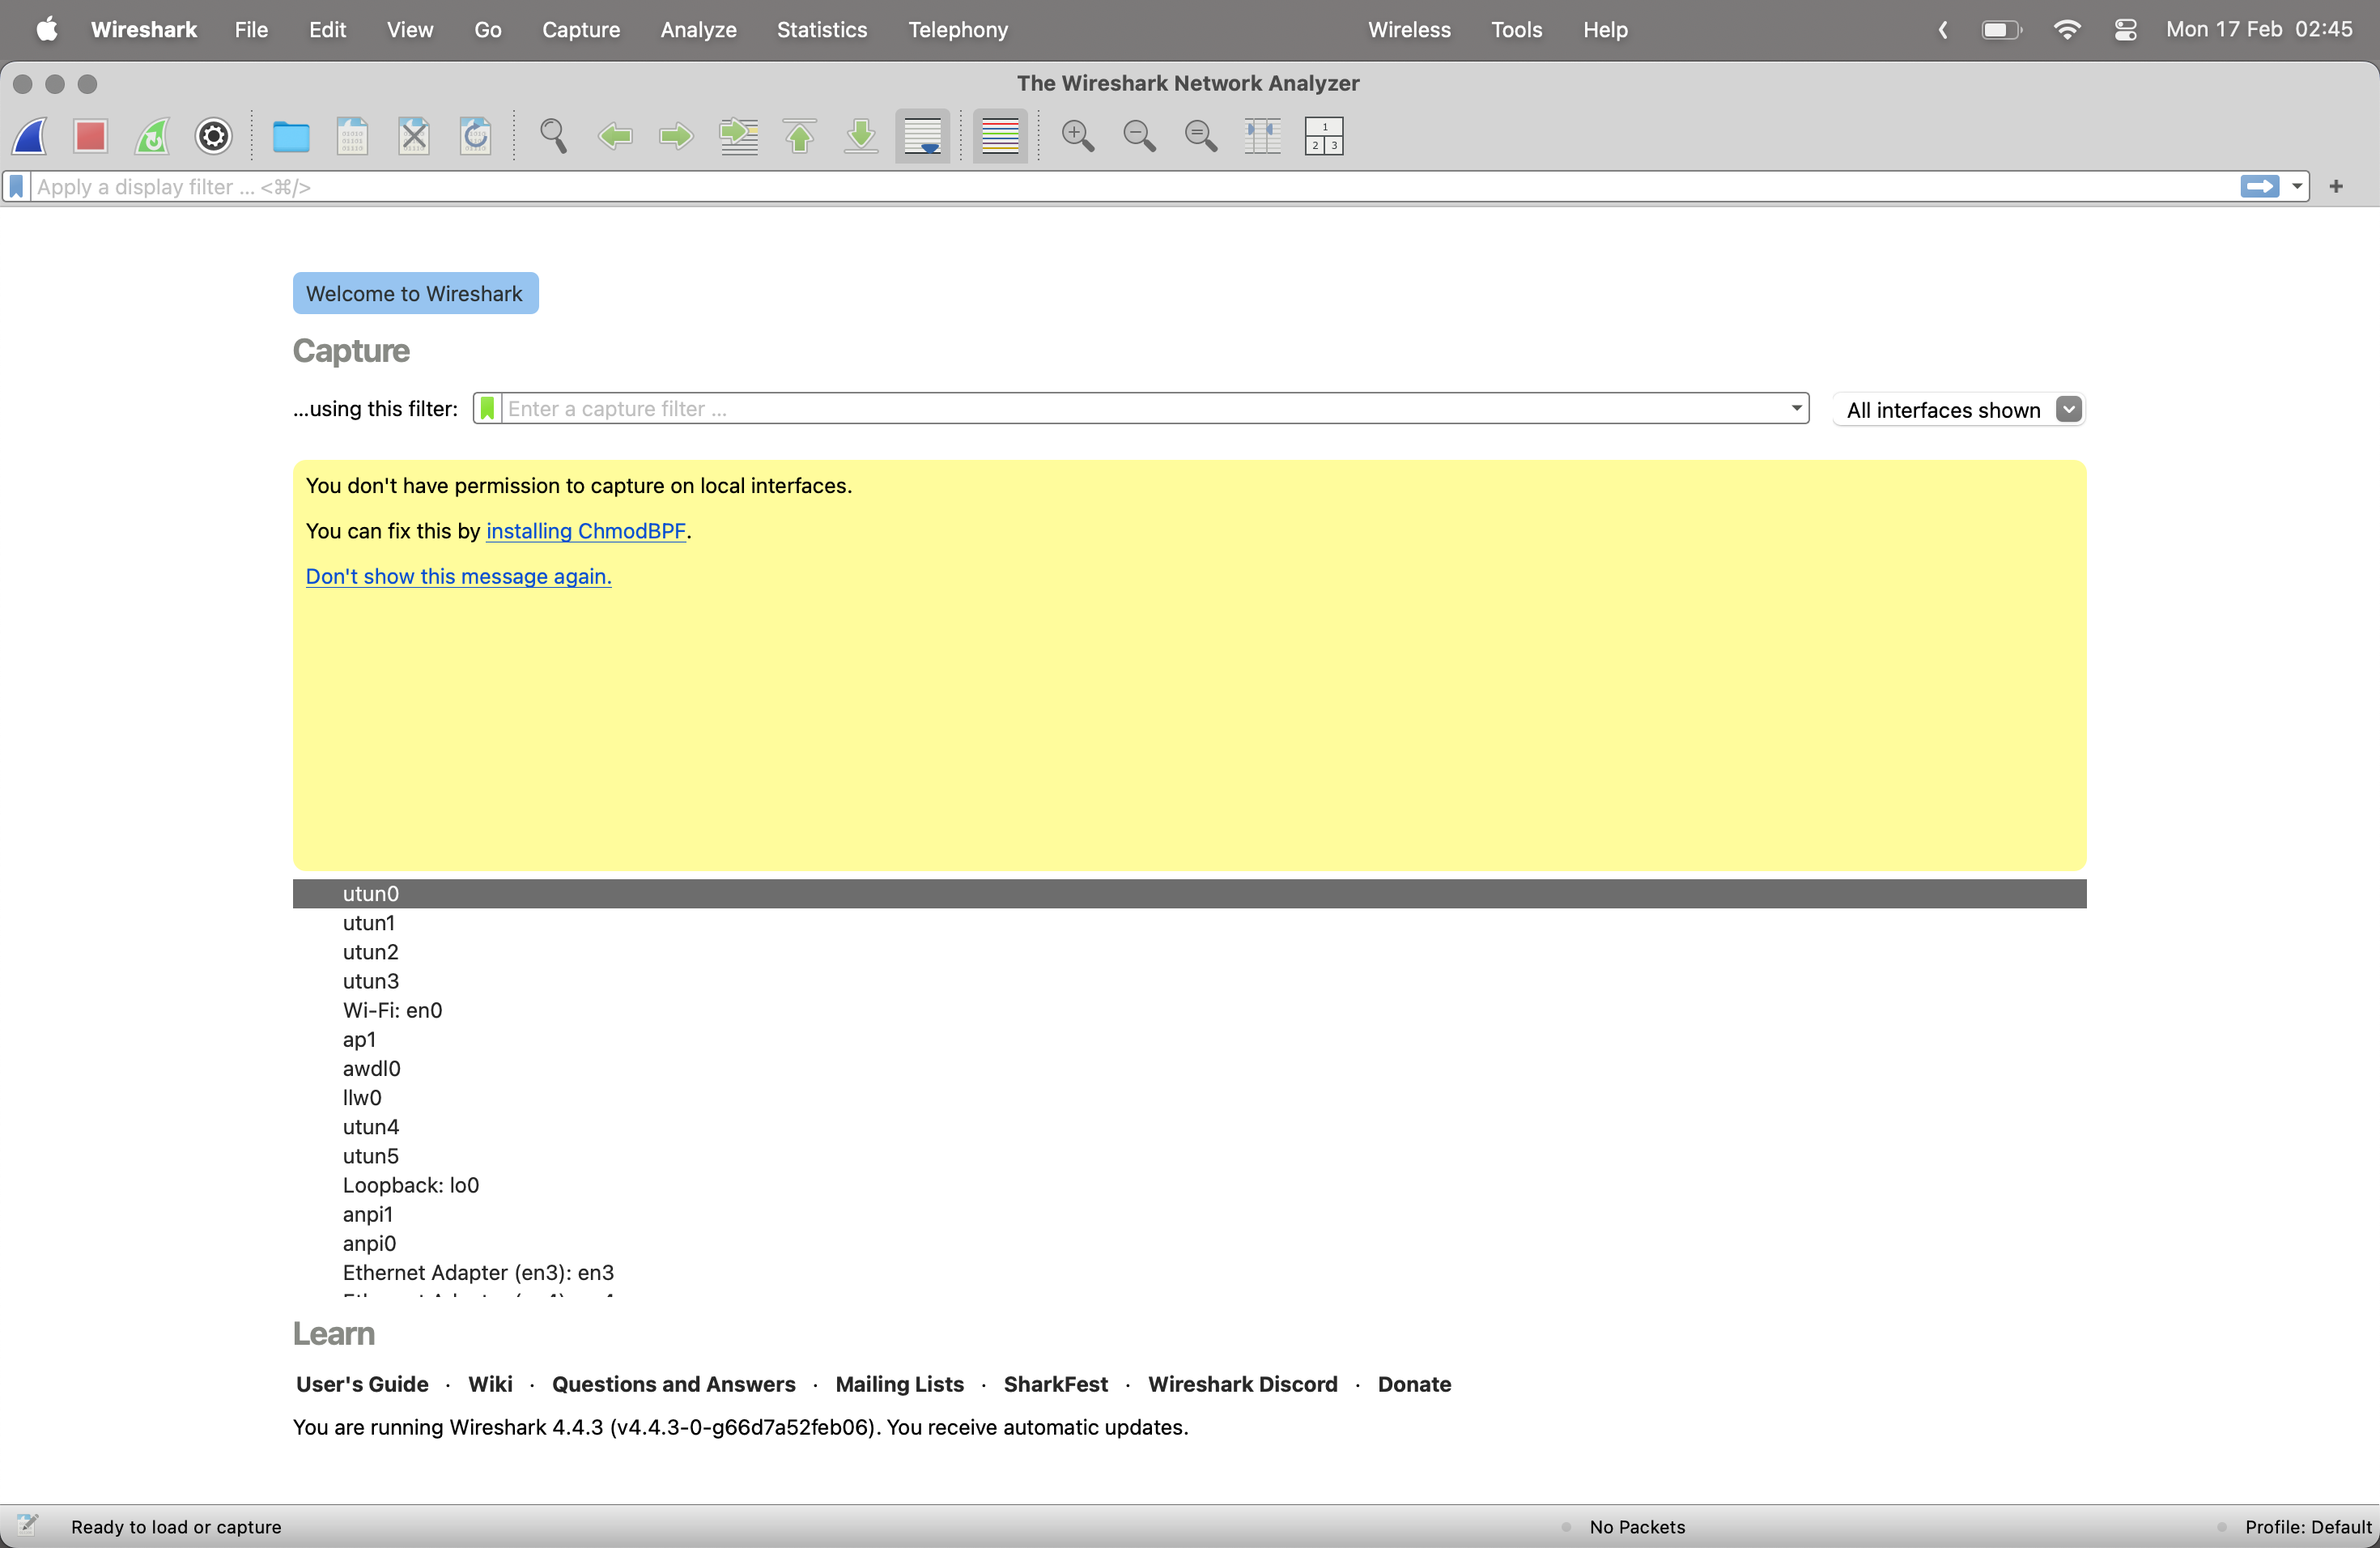
\includegraphics[width=.7\textwidth]{Image4.png} \\
\end{enumerate}

\subsection{Step 2: Capture DNS traffic.}

\begin{enumerate}
    \item Started Wireshark and click on the network interface to capture packets. \\
    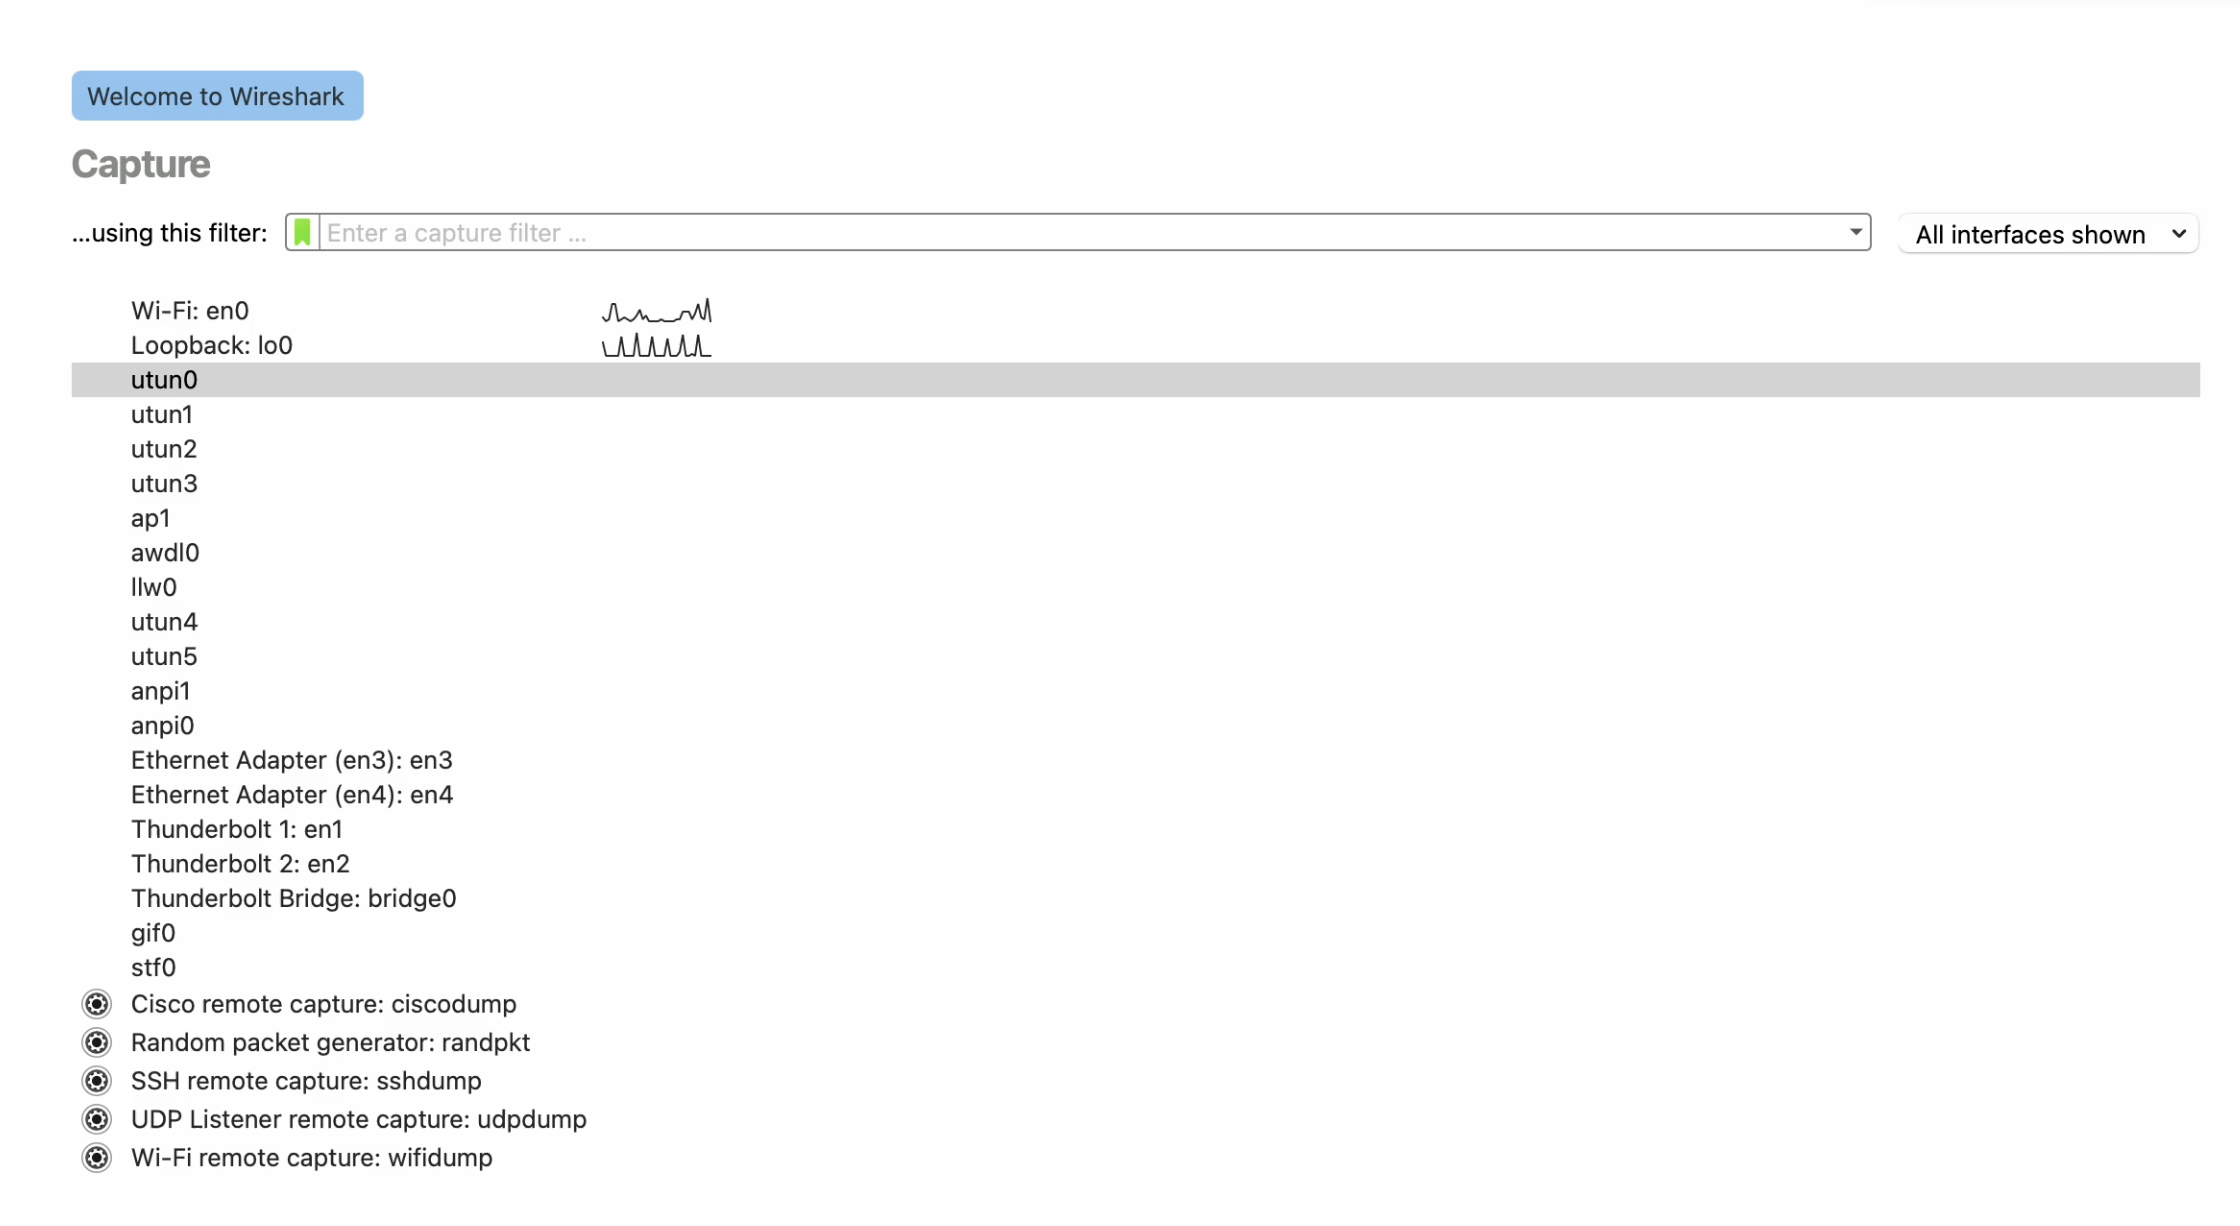
\includegraphics[width=.7\textwidth]{Image5.png} \\
    \item Clear the DNS cache.
    \begin{enumerate}
        \item Because of I have MacOS I entered the following command in the terminal: \texttt{sudo killall -HUP mDNSResponder}. \\
        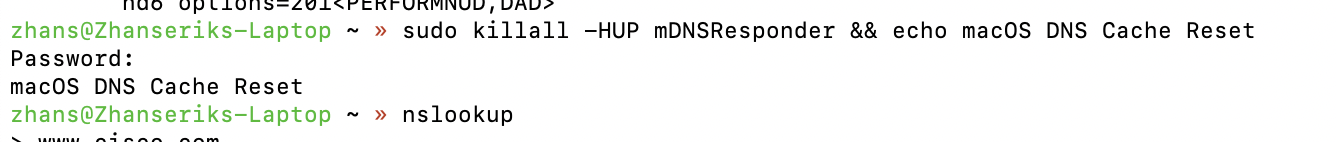
\includegraphics[width=.7\textwidth]{Image6.png} \\
    \end{enumerate}
    \item After that wrote command lookup for the domain name \texttt{www.cisco.com} in the terminal, after end of the process wrote exit. \\
    
\includegraphics[width=.7\textwidth]{Image7.png} \\
    \item Clicked \textbf{Stop capturing packets} to stop the Wireshark capture. \\
    
\includegraphics[width=.7\textwidth]{Image8.png} \\
\end{enumerate}

\section{Explore DNS Query Traffic}

\begin{enumerate}
    \item Entered \texttt{udp.port == 53} in the display filter to show only DNS traffic. \\
    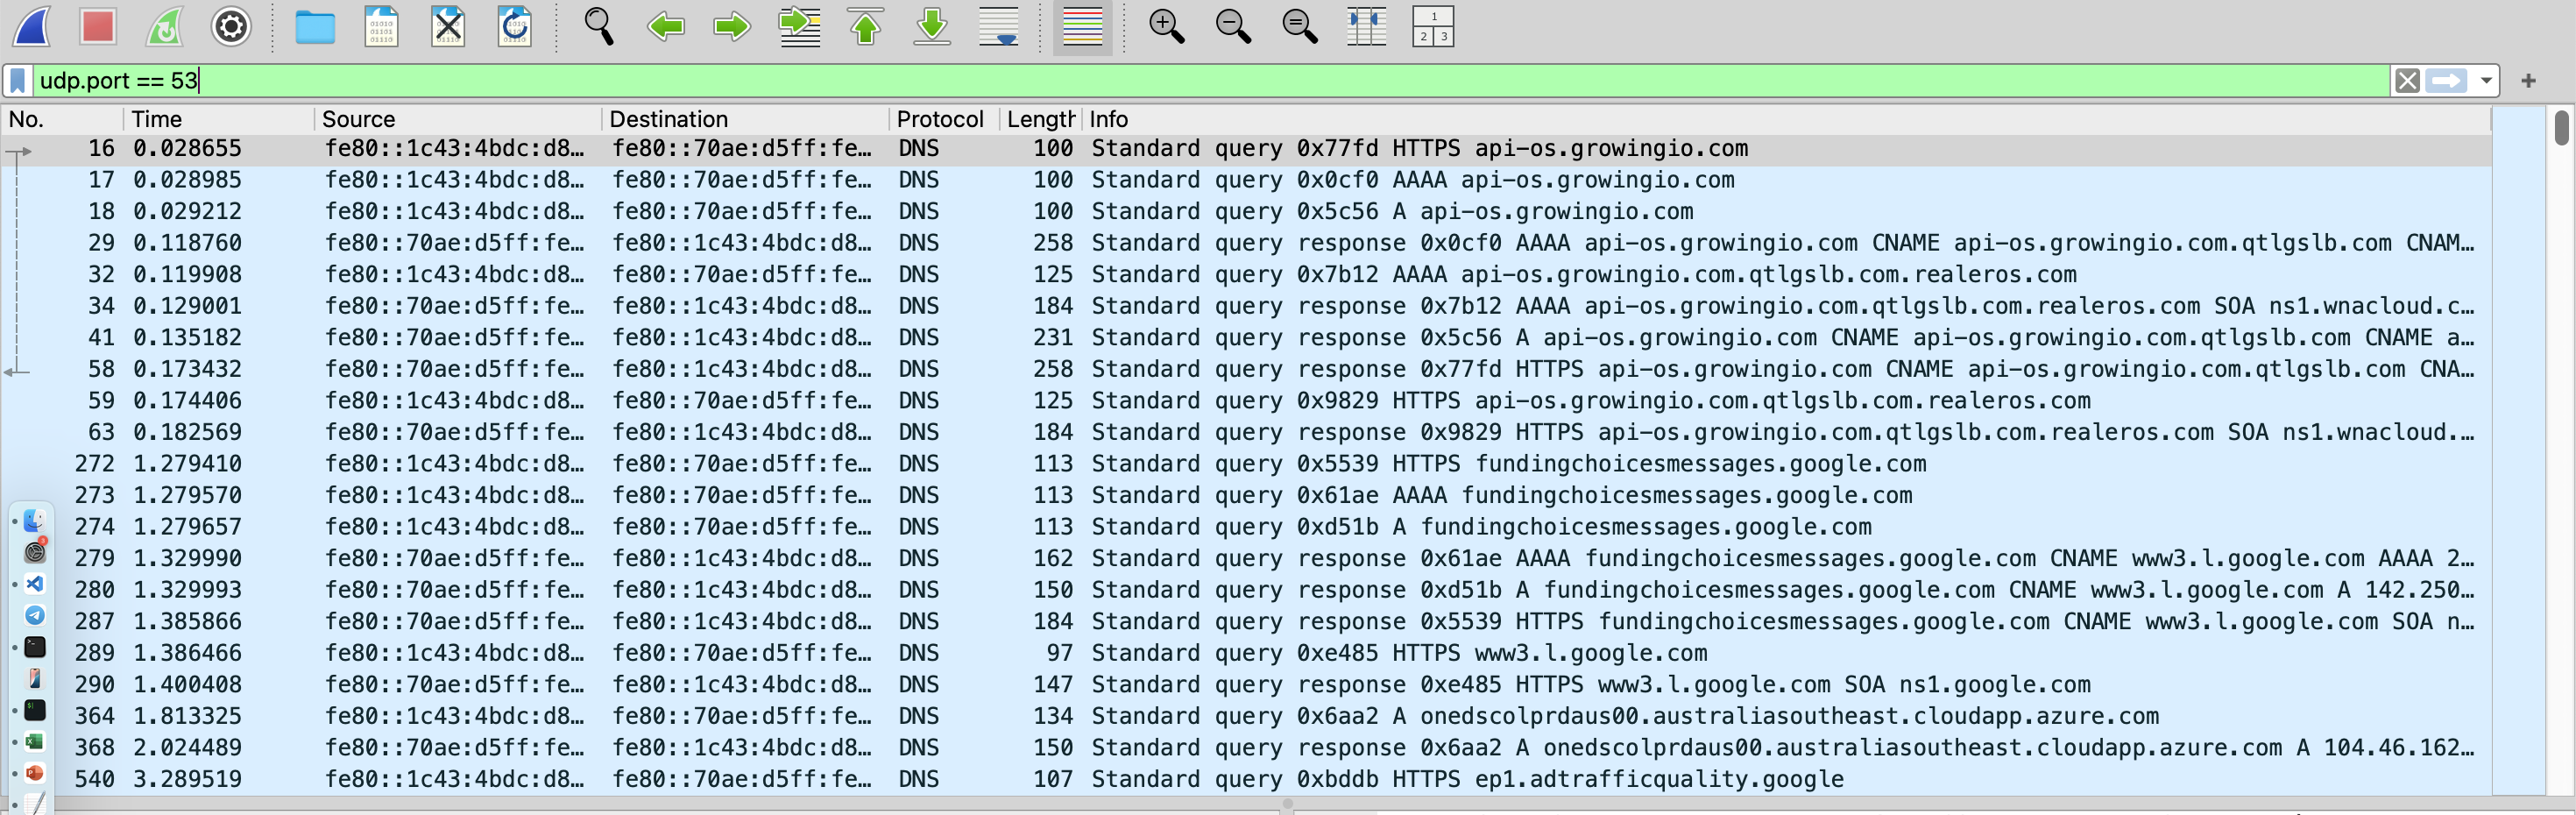
\includegraphics[width=.7\textwidth]{Image9.png} \\
    \item Selected the DNS packet contains \textbf{Standard query} and \textbf{A www.cisco.com} in the Info column. \\
    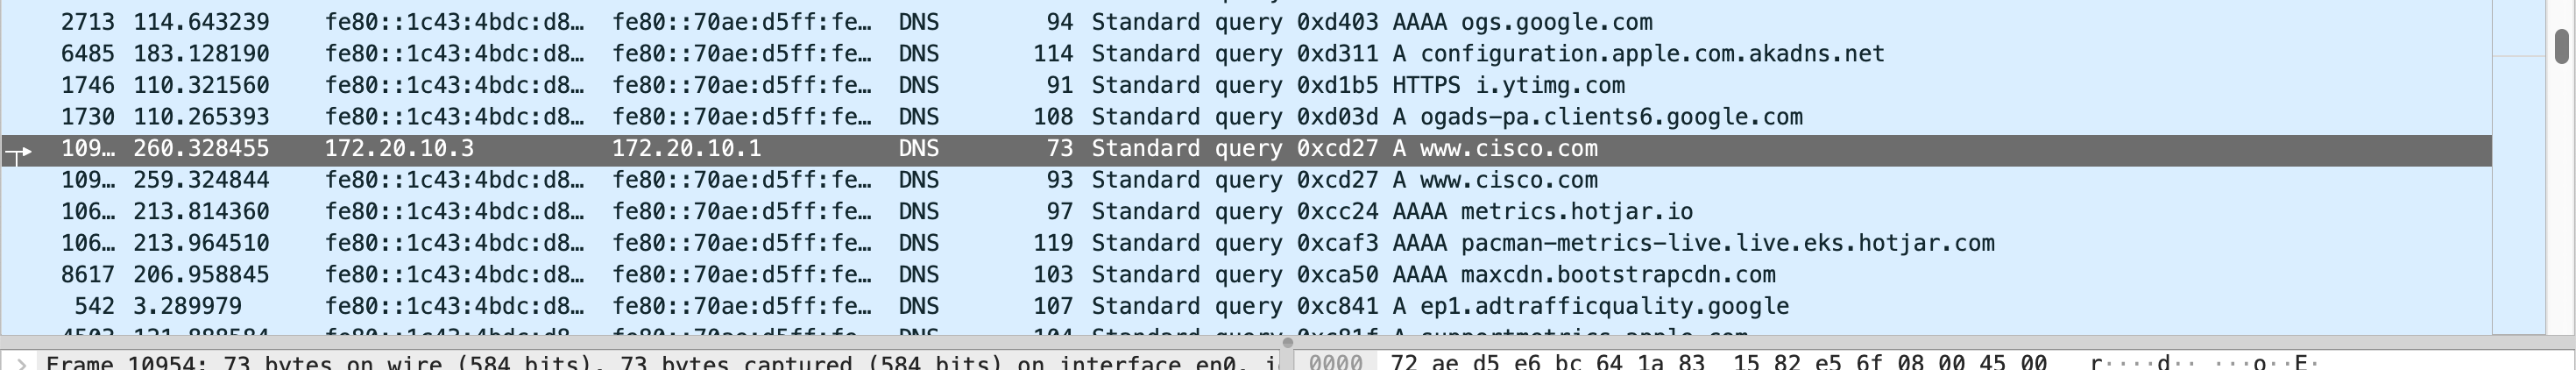
\includegraphics[width=.7\textwidth]{Image10.png} \\
    \item Details \\
    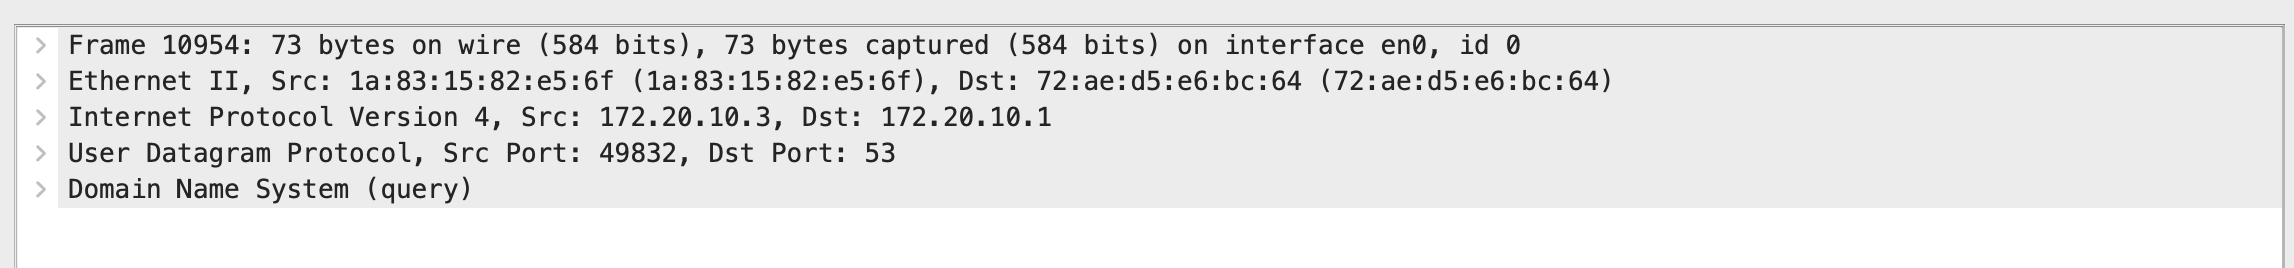
\includegraphics[width=.7\textwidth]{Image11.png} \\
    \item \textbf{Question}: What are the source and destination MAC addresses? Which network interfaces are these MAC addresses associated with? \\
    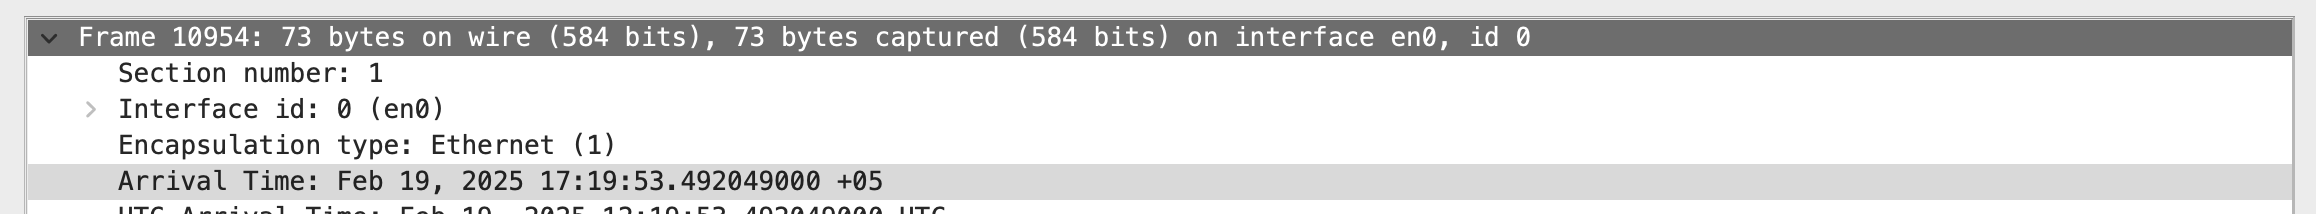
\includegraphics[width=.7\textwidth]{Image12.png} \\
    \textbf{Answer}: src: 1a:83:15:82:e5:6f, dst: 72:ae:d5:e6:bc:64, network interface en0. \\ 
    \item Expanded the \textbf{Internet Protocol Version 4}. \\
    
\includegraphics[width=.7\textwidth]{Image13.png} 
    \item \textbf{Question}: What are the source and destination IP addresses? Which network interfaces are these IP addresses associated with?  \\
    \textbf{Answer}: src: 172.20.10.3, dst: 172.20.10.1, with the interface en0.\\
    \item Expanded the \textbf{User Datagram Protocol}. \\
    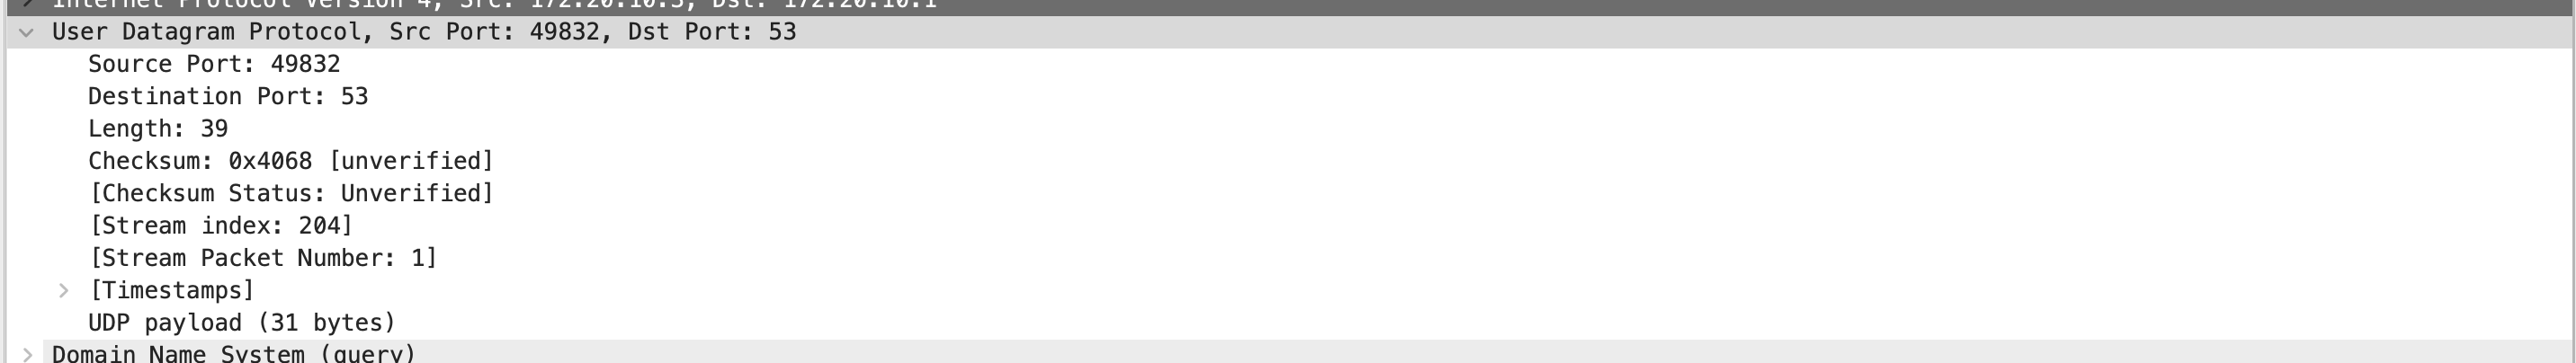
\includegraphics[width=.7\textwidth]{Image14.png} 
    \item \textbf{Question}: What are the source and destination ports? What is the default DNS port number? \\
    \textbf{Answer}: src port: 49832, dst port: 53, port number 53.\\
    \newpage
    \item Determine the IP and MAC address of the PC. 
    \begin{enumerate}
        \item Because I have MacOS, I used \texttt{ifconfig} command. \\
        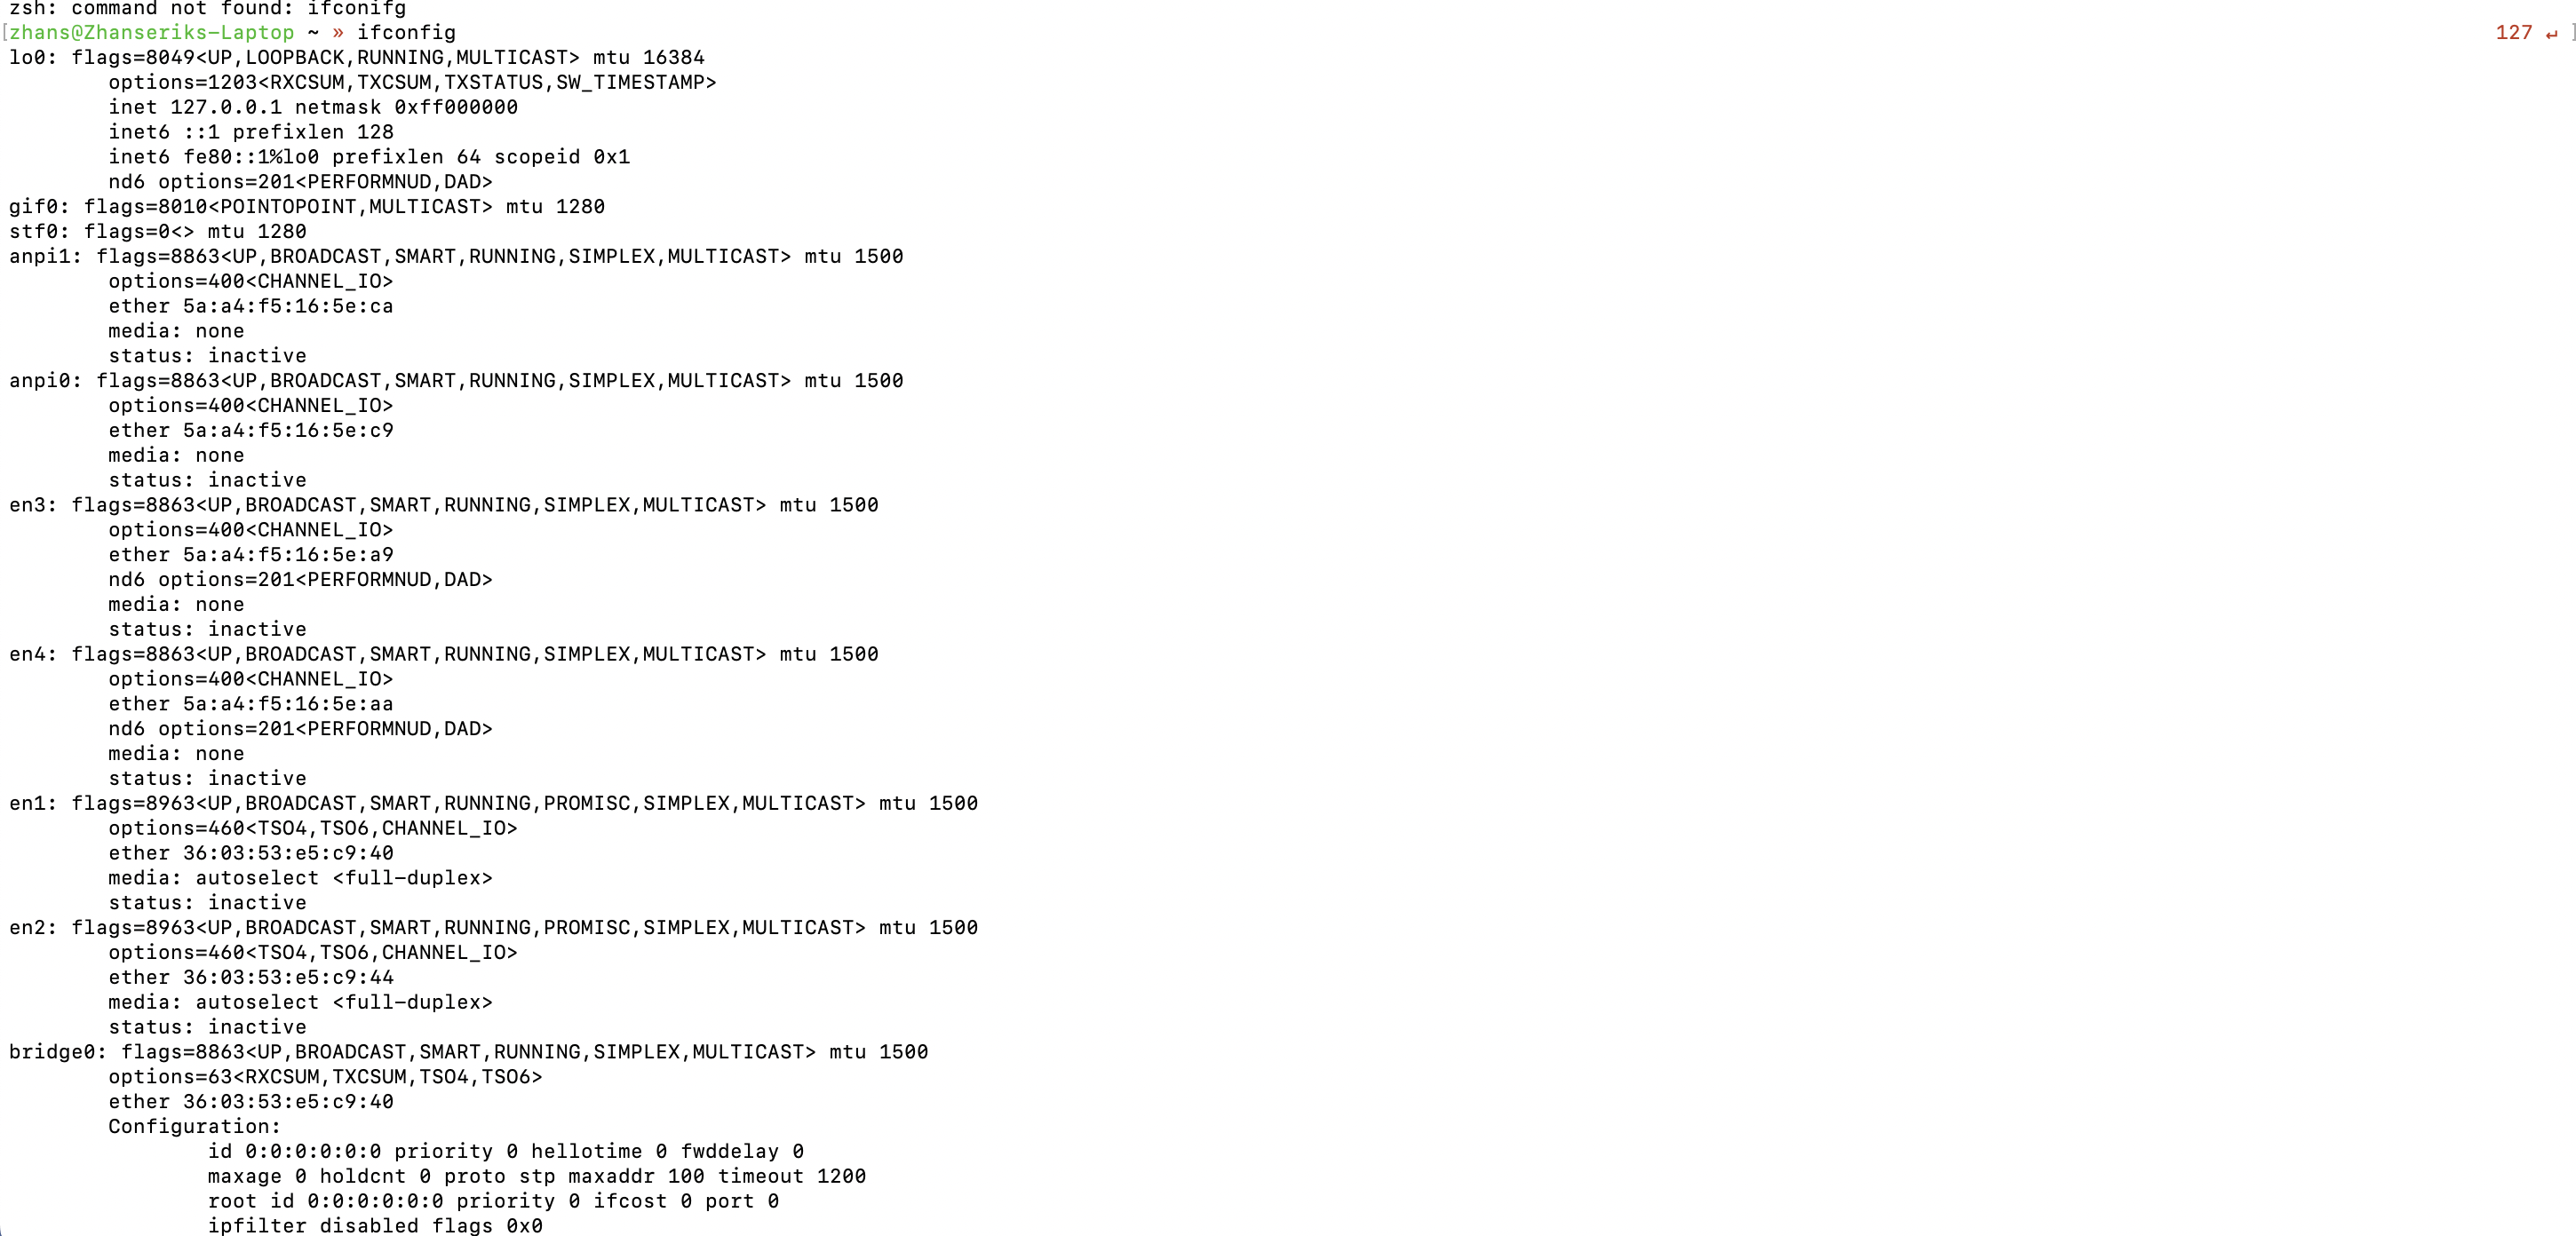
\includegraphics[width=.7\textwidth]{Image15.png}
    \end{enumerate}
    \item \textbf{Question}: Compare the MAC and IP addresses in the Wireshark results to the IP and MAC addresses What is your observation? \\
    \textbf{Answer}: I had difference in Mac addresses, but ip addresses is same.
    \item Expanded the \textbf{Domain Name System (query)} and all subsections \textbf{flags} and \textbf{queries}. \\
    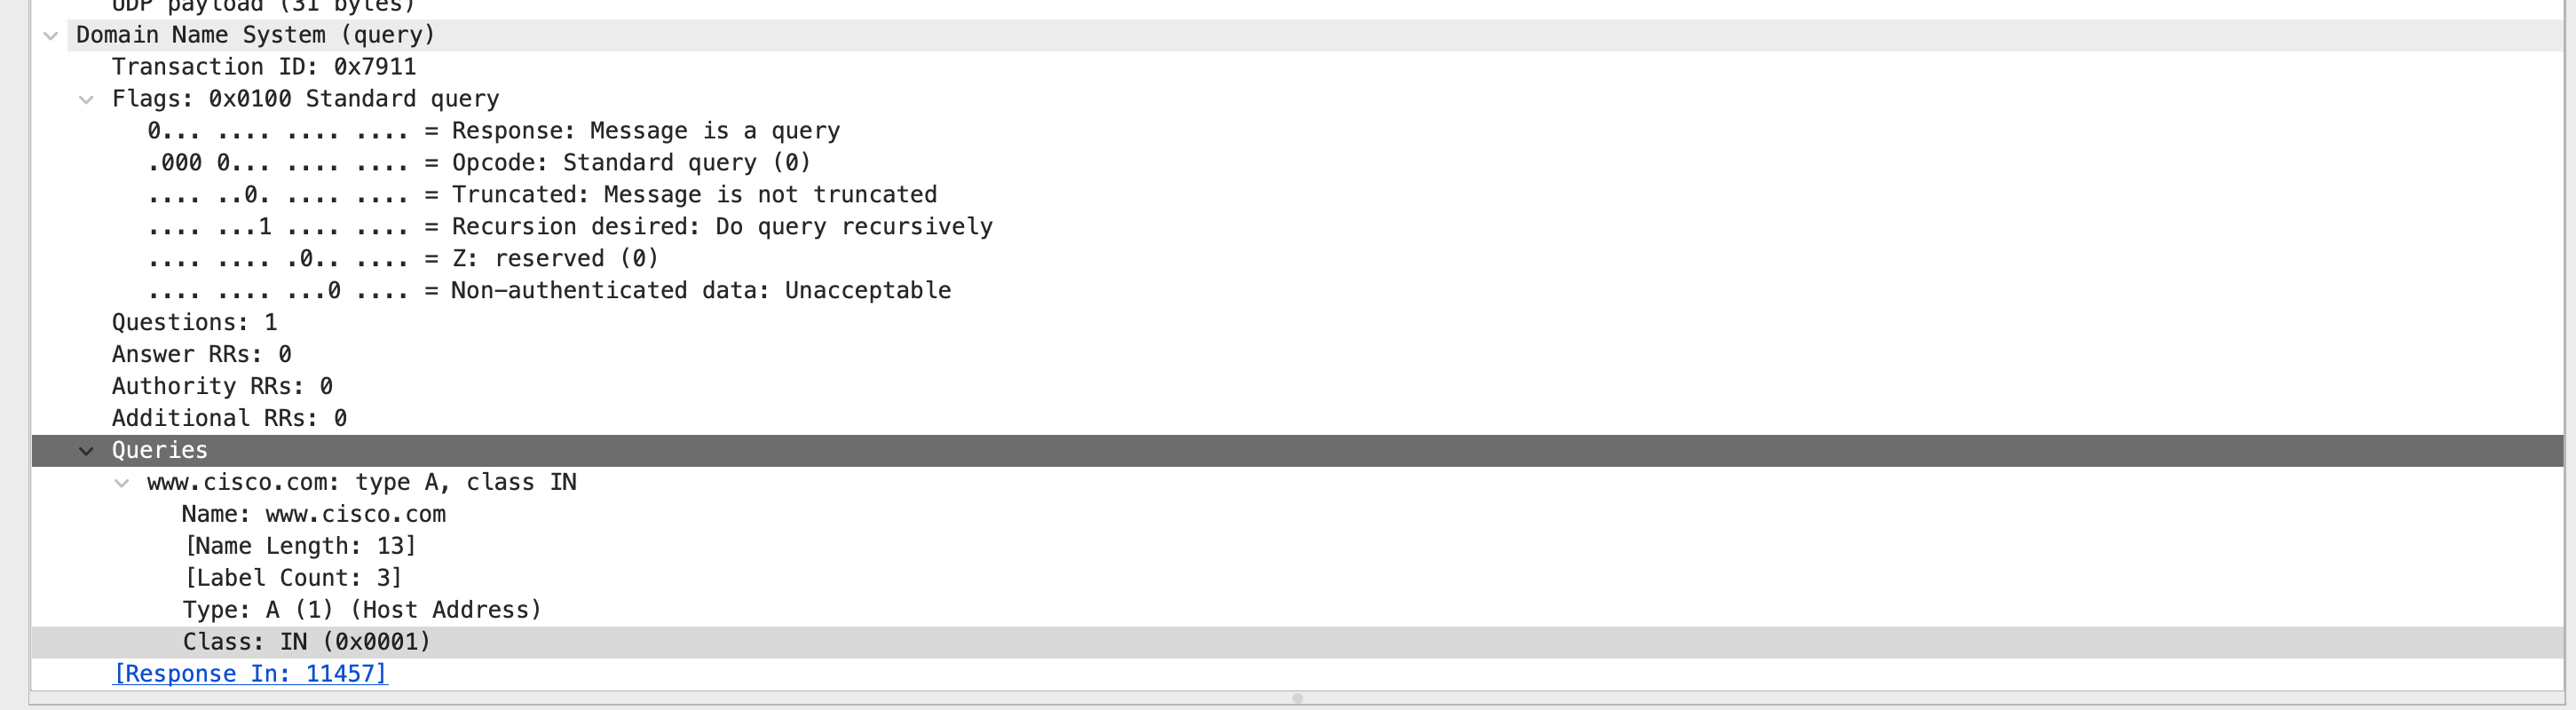
\includegraphics[width=.7\textwidth]{Image16.png}
\end{enumerate}

\section{Explore DNS Response Traffic}

\begin{enumerate}
    \item Selected the corresponding response DNS packet that has \textbf{Standard query response} and \textbf{www.cisco.com} in the Info column. \\ 
    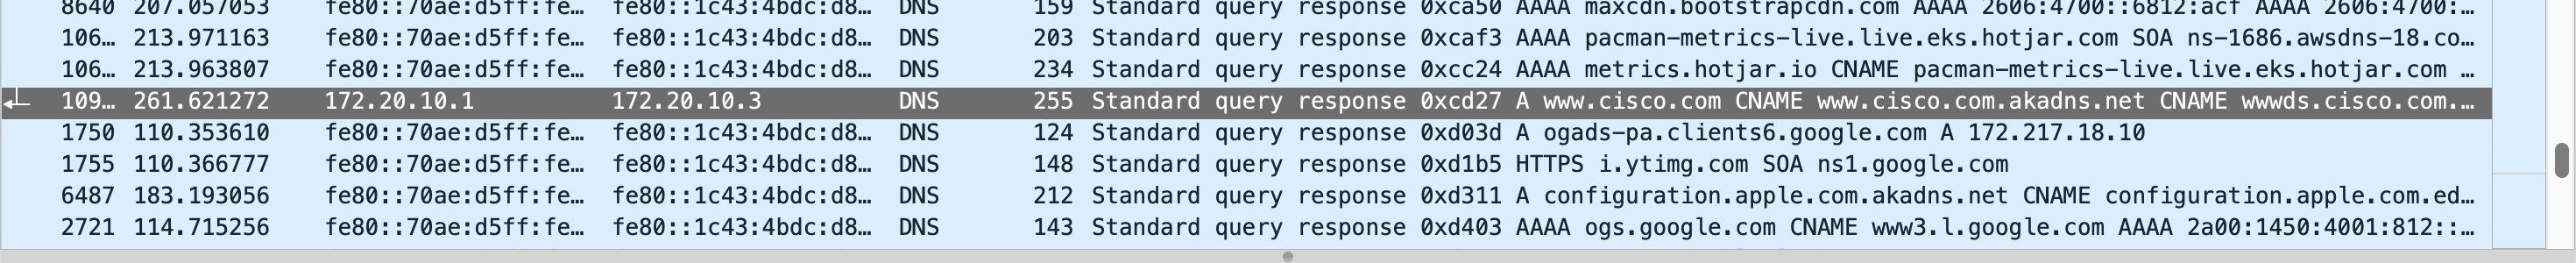
\includegraphics[width=.7\textwidth]{Image17.png} 
    \item \textbf{Question}: What are the source and destination MAC and IP addresses and port numbers? \\
    \textbf{Answer}: Mac src: 72:ae:d5:e6:bc:64 dest: 1a:83:15:82:e5:6f. IP src: 172.20.10.1 dest: 172.20.10.3. Port numbers src: 53, dest: 49832 \\
    \item How do they compare to the addresses in the DNS query packets?
    \textbf{Answer}: Same but just change the direction(src now is dest, and dest is src). \\ 
    \item Expanded \textbf{Domain Name System (response)}. [cite: 42] Then expanded the \textbf{Flags}, \textbf{Queries}, and \textbf{Answers}. \\
    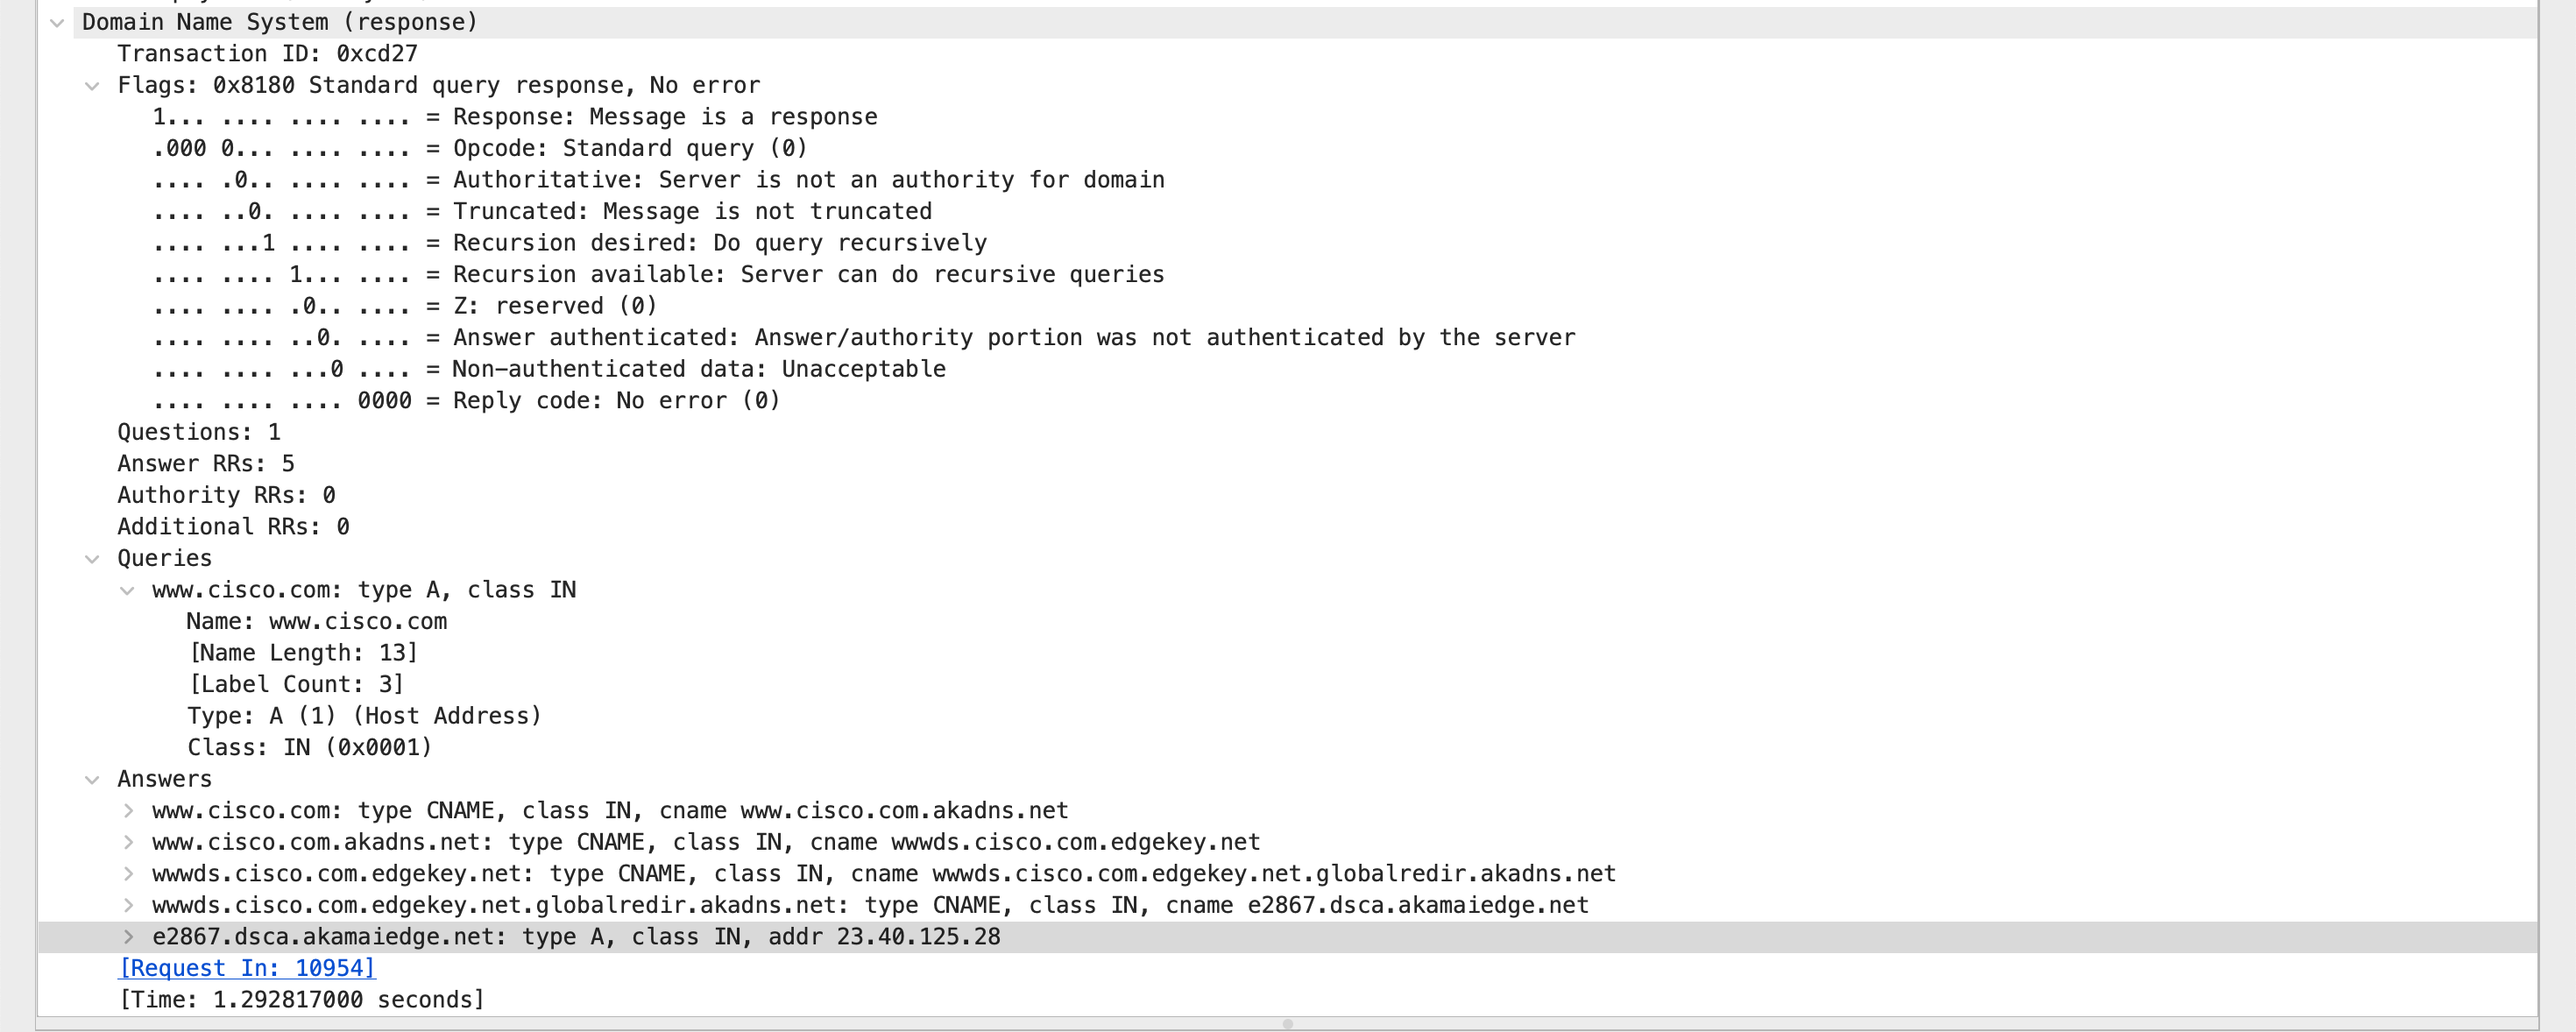
\includegraphics[width=.7\textwidth]{Image18.png} \\
    \item \textbf{Question}: Can the DNS server do recursive queries? \\ 
    \textbf{Answer}: Yes, dns server can. 
    \item Observed the CNAME and A records in the Answers details. \\
    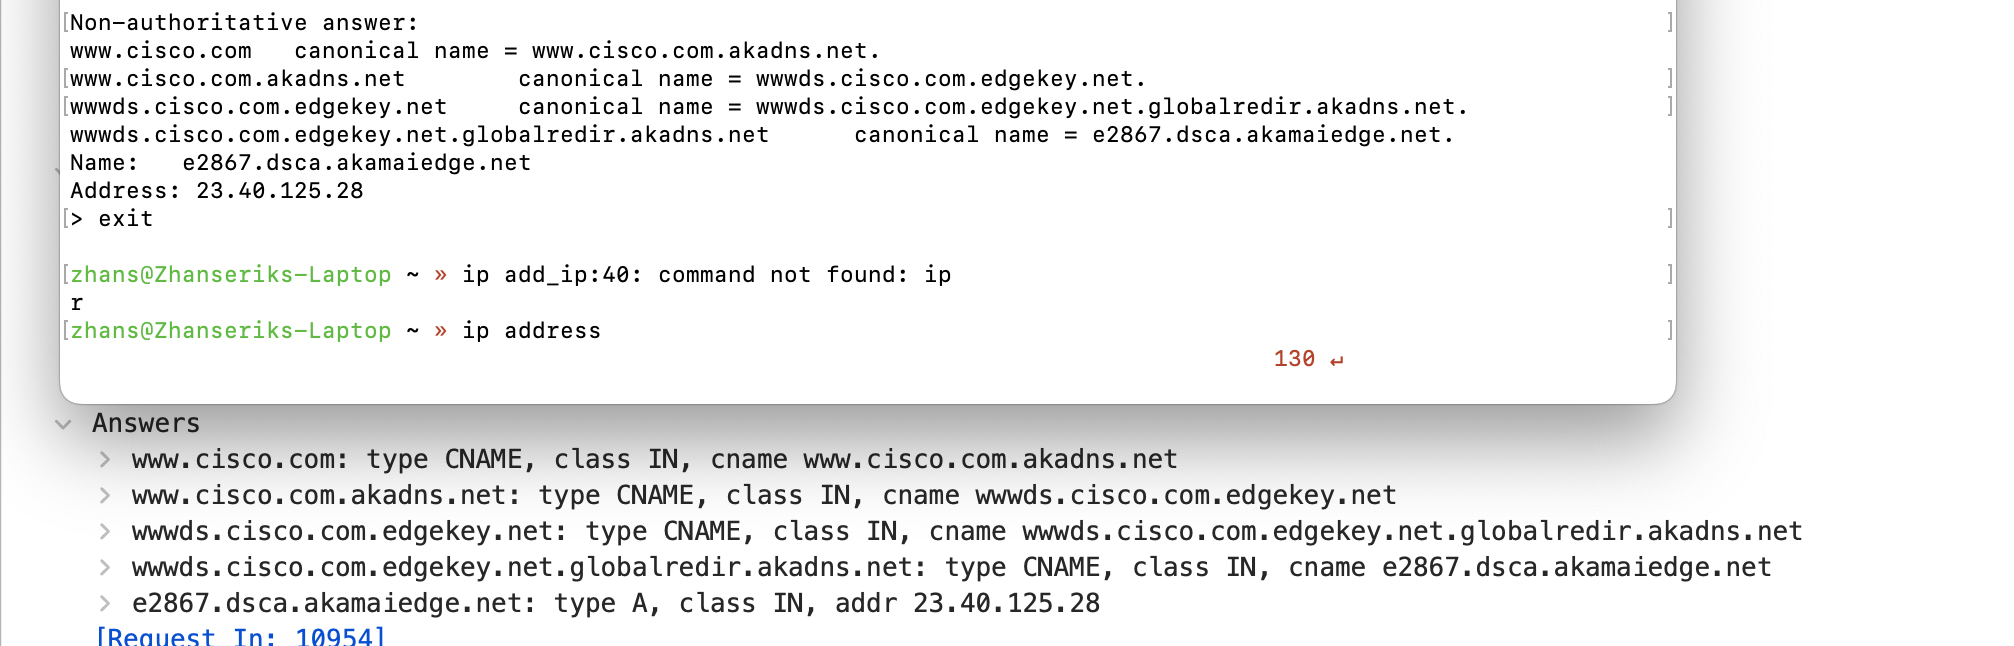
\includegraphics[width=.7\textwidth]{Image19.png} \\
    \item \textbf{Question}: How do the results compare to nslookup results? \\
    \textbf{Answer}: The same path, but with more details.
\end{enumerate}

\section{Reflection}

\begin{enumerate}
    \item From the Wireshark results, what else can you learn about the network when you remove the filter? \\
    \textbf{Answer}: Without filters, results show other packets like DHCP and ARP, revealing information about other devices and their roles in the LAN. \\
    \item How can an attacker use Wireshark to compromise your network security?  \\
    \textbf{Answer}: An attacker can use Wireshark to capture unencrypted sensitive information on the network.    
\end{enumerate}

\end{document}